\documentclass[a4paper, twoside]{ltxdoc}
\usepackage[UTF8, heading=true, scheme=plain, linespread=1.2, zihao=-4, fontset=fandol]{ctex}

% counterwith重定义问题
\let\counterwithout\relax
\let\counterwithin\relax

\usepackage{titlesec, titletoc}
\usepackage{amsfonts,amssymb} %对标题和目录操作的包
\usepackage{amsmath}% math包的扩展
\numberwithin{equation}{section} %公式自动标注
\usepackage{diagbox}% math包的扩展
\usepackage{CJK}
\usepackage{CJKulem}
\usepackage[hidelinks]{hyperref} %上面三个包对涉及中文过程的依赖包
\usepackage{geometry, parskip, seqsplit, fancyhdr, etoolbox, tocloft} %空间调整包
\usepackage{flafter, chngcntr, caption, multirow, graphicx} %处理图表的包
\usepackage{minted} % 代码高亮模块,若不需要就删去,这个视实际需要
\usepackage[bottom]{footmisc} % 脚注放到页面最底部
\usepackage[justification=centering]{caption}
\usepackage[justification=centering, list=off]{bicaption} %设置中英文标注,默认是居中,在生成图表列表下只显示第一caption的列表
\captionsetup[figure][bi-second]{name=Fig} %设置图的英文编号前缀
\captionsetup[table][bi-second]{name=Tab} %设置表的英文编号前缀

\counterwithin{figure}{section} % 图的编号按section编排
\counterwithin{table}{section} % 表的编号按section编排
\DeclareCaptionFormat{smallformat}{\songti \small #1#2#3} % 宋体,五号

% 模板设置

\newcommand{\privacy}[1][公开]{#1} % 密级
\newcommand{\type}[1][【设计或者论文】]{#1} % 类型,选填
\newcommand{\titleCna}[1][内外结合的多尺度低秩去噪算法]{#1} % 中文题目,默认最长12字符,查过部分换行到\titleCnb,我感觉大部分同学的题目长度都是超过12个字符,所以这部分我分为a,b两部分
% \newcommand{\titleCnb}[1][XXX]{#1} % 中文题目,默认最长12字符,补充到a
\newcommand{\titleEn}[1][Internal and External denoising method based on multi-scale]{#1} % 英文题目

\newcommand{\keywordsCn}[1][c语言 数据结构 论文]{#1} % 中文关键字
\newcommand{\keywordsEn}[1][c language thusis]{#1} % 英文关键字

\newcommand{\supervisor}[1][张莉\hspace{2em}教授]{#1} % 导师姓名
\newcommand{\studentID}[1][2019111238]{#1} % 学号
\newcommand{\studentNameCn}[1][韩靖敏]{#1} % 填写中文姓名
\newcommand{\studentNameEn}[1][Han Jingmin]{#1} % 填写英文姓名

\newcommand{\finishedYear}[1][2022]{#1} % 论文完成日期: 年
\newcommand{\finishedMonth}[1][04]{#1} % 论文完成日期: 月
\newcommand{\finishedDay}[1][01]{#1} % 论文完成日期: 日


\newcommand{\department}[1][数学学院]{#1} % 系名称
\newcommand{\major}[1][计算数学]{#1} % 专业名称
\newcommand{\enrolmentYear}[1][【2019级】]{#1} % 入学年份
\newcommand{\object}[1][图像去噪]{#1} %研究方向



% 字号设置
\newcommand{\chuhao}{\fontsize{42pt}{\baselineskip}\selectfont}     % 字号设置
\newcommand{\xiaochuhao}{\fontsize{36pt}{\baselineskip}\selectfont} % 字号设置
\newcommand{\yichu}{\fontsize{32pt}{\baselineskip}\selectfont}      % 字号设置
\newcommand{\yihao}{\fontsize{28pt}{\baselineskip}\selectfont}      % 字号设置
\newcommand{\erhao}{\fontsize{21pt}{\baselineskip}\selectfont}      % 字号设置
\newcommand{\xiaoerhao}{\fontsize{18pt}{\baselineskip}\selectfont}  % 字号设置
\newcommand{\sanhao}{\fontsize{15.75pt}{\baselineskip}\selectfont}  % 字号设置
\newcommand{\sihao}{\fontsize{14pt}{\baselineskip}\selectfont}      % 字号设置
\newcommand{\xiaosihao}{\fontsize{12pt}{\baselineskip}\selectfont}  % 字号设置
\newcommand{\wuhao}{\fontsize{10.5pt}{\baselineskip}\selectfont}    % 字号设置
\newcommand{\xiaowuhao}{\fontsize{9pt}{\baselineskip}\selectfont}   % 字号设置
\newcommand{\liuhao}{\fontsize{7.875pt}{\baselineskip}\selectfont}  % 字号设置
\newcommand{\qihao}{\fontsize{5.25pt}{\baselineskip}\selectfont}    % 字号设置
\newcommand{\fighao}{\fontsize{11pt}{\baselineskip}\selectfont}    % 字号设置

% 下划线
\newcommand{\underlineFixlen}[2][3.5cm]{\underline{\makebox[#1][c]{#2}}}


% 中文摘要
\renewenvironment{abstract}{
%\thispagestyle{empty} % 去掉页码
{
\begin{center}
\Large \songti \bfseries 摘\hspace{1em}要\vspace{1.1cm}
\end{center}
}
\setlength{\parindent}{2em}
\setlength{\parskip}{0em}
\setlength{\lineskip}{0em} 
\setlength{\baselineskip}{20pt} % (宋体,小四;固定行距22磅,段前、段后均为0行间距。段落首行缩进2字符。)
\songti
}{
\setlength{\parindent}{0em}
\setlength{\parskip}{1em}
{\par \songti \bfseries{关键词:}}
\keywordsCn
\clearpage
}

% 英文摘要
\newenvironment{abstractEn}{
%\thispagestyle{empty} % 去掉页码
{
\begin{center}
\Large \bfseries ABSTRACT\vspace{1.5cm}
\end{center}
}
\setlength{\parindent}{2em}
\setlength{\parskip}{0em}
\setlength{\lineskip}{0em} 
\setlength{\baselineskip}{20pt} % 22磅行距,首行缩进1字符,段前、段后均为0行间距
}{
\setlength{\parindent}{0em}
\setlength{\parskip}{1em}
{\par \bfseries{KEYWORDS: }}
\keywordsEn
\clearpage
}

% 目录名
\renewcommand\contentsname{
\begin{center}
\songti \Large \bfseries 目\hspace{1em}录 % (宋体,小二号,加粗;居中,单倍行距,段前0.5行、段后1.5行间距)
\end{center}
\vspace{1em}
}
% 插图清单
\renewcommand\listfigurename{
\begin{center}
\songti \Large \bfseries 插图清单 % (宋体,小二号,加粗;居中,单倍行距,段前0.5行、段后1.5行间距)
\end{center}
\vspace{1em}
}

% 表格清单
\renewcommand\listtablename{
\begin{center}
\songti \Large \bfseries 表格清单 % (宋体,小二号,加粗;居中,单倍行距,段前0.5行、段后1.5行间距)
\end{center}
\vspace{1em}
}

\renewcommand\refname{\heiti \sanhao \bfseries 参考文献}


% 目录引线设置
\renewcommand{\cftdotsep}{1.5} % 线的密度
\renewcommand{\cftsecdotsep}{1.5} % section引线
\renewcommand{\cftsecleader}{\cftdotfill{\cftsecdotsep}}
\renewcommand{\cftsecpagefont}{}

% 插图清单
\renewcommand{\cftfigpresnum}{\figurename\enspace}

% 表格清单
\renewcommand{\cfttabpresnum}{\tablename\enspace}

% 致谢
\newenvironment{acknowledge}{
\clearpage
\vspace*{-2em}
%\phantomsection % 使得hyperref目录能够跳转到正确的位置
%\addcontentsline{toc}{section}{致谢} % 添加到目录中
\begin{center}
 \songti \Large \bfseries 致谢\end{center}\vspace{1.1cm}
\setlength{\parindent}{2em}
\setlength{\parskip}{0em}
\setlength{\lineskip}{0em} 
\setlength{\baselineskip}{20pt} % (宋体,小四;固定行距22磅,段前、段后均为0行间距。段落首行缩进2字符。)
\songti
\par
}{
	\par
	\hfill 作者:\studentNameCn

	\hfill \finishedYear\enspace 年\finishedMonth\enspace 月\finishedDay\enspace 日
}

% 攻读硕士学位期间的学术活动及成果情况
\newenvironment{achievement}{
\clearpage
\vspace*{-2em}
\phantomsection % 使得hyperref目录能够跳转到正确的位置
\addcontentsline{toc}{section}{攻读硕士学位期间的学术活动及成果情况} % 添加到目录中
\begin{center}
\songti \Large \bfseries 攻读硕士学位期间的学术活动及成果情况\end{center}\vspace{1.1cm}
\setlength{\parindent}{0em}
\setlength{\parskip}{0em}
\setlength{\lineskip}{0em} 
\setlength{\baselineskip}{20pt} % (宋体,小四;固定行距22磅,段前、段后均为0行间距。段落首行缩进2字符。)
\heiti
\par
}

% 附录
\renewenvironment{appendix}{
\clearpage
\vspace*{-2em}
\phantomsection % 使得hyperref目录能够跳转到正确的位置
\addcontentsline{toc}{section}{附录} % 添加到目录中
\begin{center}
 \songti \Large \bfseries 附录\end{center}\vspace{1.1cm}
\setlength{\parindent}{2em}
\setlength{\parskip}{0.5em}
\setlength{\baselineskip}{22pt} % 22磅行距,首行缩进1字符,段前、段后均为0行间距
\songti
\par
}{
}

% 图名称
\renewcommand{\figurename}{图}
\renewcommand{\tablename}{表}


\captionsetup{
	labelsep=quad, % caption去掉分隔符:
	textformat=simple,
	format=smallformat,
}

\titleformat{\section}{\centering \heiti \sanhao \bfseries}{第\chinese{section}章}{0.5em}{}

% 根据毕业要求设置字体
\ctexset{
	space=auto,
	section = {
		format = \centering \heiti \sanhao \bfseries,
		aftername = \hspace{1em}, 
		afterindent = true,
	},
	subsection = {
		format = \heiti \xiaosihao \bfseries,
		aftername = \hspace{0.4em},
		afterindent = true,
	},
	subsubsection = {
		format = \songti \xiaosihao \bfseries,
		aftername = \hspace{0.4em},
		afterindent = true,
	},
}

%一级标题段前段后单倍行距,二级、三级等标题为0.5倍行距,只做到subsub标题,如果需要依次加入即可
\titlespacing{\section} {0pt}{12pt}{12pt}
\titlespacing{\subsection} {0pt}{6pt}{6pt}
\titlespacing{\subsubsection} {0pt}{6pt}{6pt}

\geometry{left=3cm, right=3cm, top=2.54cm, bottom=2.54cm} %按照格式要求左右3cm,上下2.54cm

\titlecontents{section}[0pt]{\addvspace{1.5pt}\filright\bf}%
               {\contentspush{\thecontentslabel \quad}}%
               {}{\titlerule*[8pt]{.}\contentspage}
             
\CTEXsetup[name={第,章},number={\chinese{section}}]{section} %上面几句用于操作目录

\setmainfont{Times New Roman} % 英文字体

\begin{document}
\begin{titlepage}
{
\heiti 单位代码:\underlineFixlen[3.5cm]{} \hfill 
{\heiti 密\hspace{1.3em}级:\underlineFixlen[3.5cm]{\privacy}} \\
\heiti 学\hspace{2em}号:\underlineFixlen[3.5cm]{\studentID} \hfill
{\heiti 分类号:\underlineFixlen[3.5cm]{}}	
}

\centering
{\vspace{1.7cm} 
\includegraphics{images/hfut_name.png}\vspace{0.3cm}}

{
\parskip=0.5em
\linespread{1.25}

{\LARGE \bfseries Hefei University of Technology}\vspace{1cm}

{\chuhao \heiti 硕士学位论文}\vspace{0.7cm}

{\LARGE  \bfseries MASTER'S DISSERTATION}\vspace{0.4cm}

{\LARGE \bfseries (学术硕士)}\vspace{3cm}

}


{
\linespread{1.6}
\songti \sanhao
	{论文题目:}\underlineFixlen[8.8cm]{\titleCna}\\
	{\hspace{4.8em}} \underlineFixlen[8.8cm]{\titleCnb}\\
	{学科专业:}\underlineFixlen[8.8cm]{\major}\\
	{学生姓名:}\underlineFixlen[8.8cm]{\studentNameCn}\\
	{导师姓名:}\underlineFixlen[8.8cm]{\supervisor}\\
	{完成时间:}\underlineFixlen[8.8cm]{\finishedYear 年\finishedMonth 月}\\
}


\end{titlepage}

\begin{titlepage}
\centering

{
\parskip=0.5em
\linespread{1.25}
\LARGE \heiti
合\hspace{1.5em}肥\hspace{1.5em}工\hspace{1.5em}业\hspace{1.5em}大\hspace{1.5em}学\vspace{1.5cm}

{\heiti 学历硕士学位论文}\vspace{1.5cm}

\centering\songti \bfseries{\titleCna} \\
\centering\songti \bfseries{\titleCnb} \vspace{6cm}

}

{
\parskip=0.5em \linespread{1.5}
\songti \sanhao
作者姓名:\underlineFixlen[8.8cm]{\studentNameCn}

指导教师:\underlineFixlen[8.8cm]{\supervisor}

学科专业:\underlineFixlen[8.8cm]{\major}

研究方向:\underlineFixlen[8.8cm]{\object}

\vspace{3.2cm}
\large
\finishedYear 年\finishedMonth 月
}


\end{titlepage}

\begin{titlepage}
\centering
{
\parskip=0pt \linespread{1.25}
\sanhao {A Dissertation Submitted for the Degree of Bachelor}\vspace{4.7cm}

\Large \bfseries{\titleEn} \vspace{1.8cm}}

{\sanhao By

\studentNameEn
\vfill
Hefei University of Technology

Hefei, Anhui, P.R.China

\finishedMonth ,\enspace \finishedYear
\vspace{3cm}
}

\end{titlepage}

\begin{titlepage}
\setlength{\parindent}{2em}
\setlength{\parskip}{0.5em}

{
\begin{center}
\heiti \Large
	\bfseries{毕业设计(论文)独创性声明}\vspace{1.2cm}
\end{center}
}

{
本人郑重声明:所呈交的毕业设计(论文)是本人在指导教师指导下进行独立研究工作所取得的成果。据我所知,除了文中特别加以标注和致谢的内容外,设计(论文)中不包含其他人已经发表或撰写过的研究成果,也不包含为获得\underlineFixlen[3cm]{合肥工业大学}或其他教育机构的学位或证书而使用过的材料。对本文成果做出贡献的个人和集体,本人已在设计(论文)中作了明确的说明,并表示谢意。

毕业设计(论文)中表达的观点纯属作者本人观点,与合肥工业大学无关。\vspace{1cm}

毕业设计(论文)作者签名:\hfill 签名日期:\hspace{2em}年\hspace{2em}月\hspace{2em}日
}

{
\vspace{3cm}
\begin{center}
\heiti \Large
	\bfseries{毕业设计(论文)版权使用授权书}\vspace{1.2cm}
\end{center}
}

{
本学位论文作者完全了解\underlineFixlen[3cm]{合肥工业大学}有关保留、使用毕业设计(论文)的规定,即:除保密期内的涉密设计(论文)外,学校有权保存并向国家有关部门或机构送交设计(论文)的复印件和电子光盘,允许设计(论文)被查阅或借阅。本人授权\underlineFixlen[3cm]{合肥工业大学}可以将本毕业设计(论文)的全部或部分内容编入有关数据库,允许采用影印、缩印或扫描等复制手段保存、汇编毕业设计(论文)。

(保密的毕业设计(论文)在解密后适用本授权书) \vspace{1.5cm}

学位论文作者签名:\hfill 指导教师签名:\hspace{7em}

签名日期:\hspace{2em}年\hspace{2em}月\hspace{2em}日\hfill 签名日期:\hspace{2em}年\hspace{2em}月\hspace{2em}日
}


\end{titlepage}

\pagenumbering{Roman} %对正文前利用罗马5号数字打页码

% 致谢
\pagestyle{plain} % 这部分不需要页眉
\begin{acknowledge}
这部分是致谢
\end{acknowledge}
\clearpage

\begin{abstract}
这部分是摘要
\end{abstract}

\begin{abstractEn}
This is English abstract.
\end{abstractEn}

% 目录
{
%\tocloftpagestyle{empty}
\setlength{\cftfignumwidth}{3.5em}
\setlength{\cfttabnumwidth}{3.5em}
\setlength{\parskip}{0em} % 段落间无空行
\setlength{\lineskip}{0em} % 行距为0,值得是每行之间固定行间距
\setlength{\baselineskip}{20pt} %行间距20磅
\clearpage

\tableofcontents
%\addtocontents{toc}{\protect\thispagestyle{empty}}
%\pagenumbering{gobble}

\clearpage
\listoffigures %插图清单

\clearpage
\listoftables %表格清单

%\pagenumbering{arabic}
}
% 设置页眉
\newgeometry{left=2.8cm, right=2.8cm, top=3cm, bottom=3cm}
\fancyhead{}                            
\fancyhead[CE]{{\songti \wuhao} 合肥工业大学学术硕士研究生学位论文 \vspace{0.3cm}} %根据以往的形式奇数页的页眉为学位论文,偶数页为章节名
\fancyhead[CO]{{\songti \wuhao} 第\chinese{section}章 \leftmark \vspace{0.3cm}}
\cfoot{\thepage} 
\pagestyle{fancy} 

% 正文
{
\setcounter{page}{1}
\pagenumbering{arabic}
% 重写section指令以便设置section段前1行间距,分页
\pretocmd{\section}{\clearpage \vspace*{-2.0em}}{}{}

\setlength{\parindent}{2em} %首行缩紧2字符
\setlength{\parskip}{0em} % 段落间无空行
\setlength{\lineskip}{0em} % 行距为0,值得是每行之间固定行间距
\setlength{\baselineskip}{20pt} %行间距20磅

\section{这是第一章}
\subsection{这是第一节}
这部分写你的文章,section为一级标题,subsection为二级标题,subsubsection为三级标题,依次类推

\begin{figure}[!htb]
	\centering
	%\vspace{-0.5cm}  %调整图片与上文的垂直距离,视情况而定,这部分我给注释掉,需要的自己加入
	%\setlength{\abovecaptionskip}{0.2cm}   %调整图片标题与图距离,视情况而定,这部分我给注释掉,需要的自己加入
	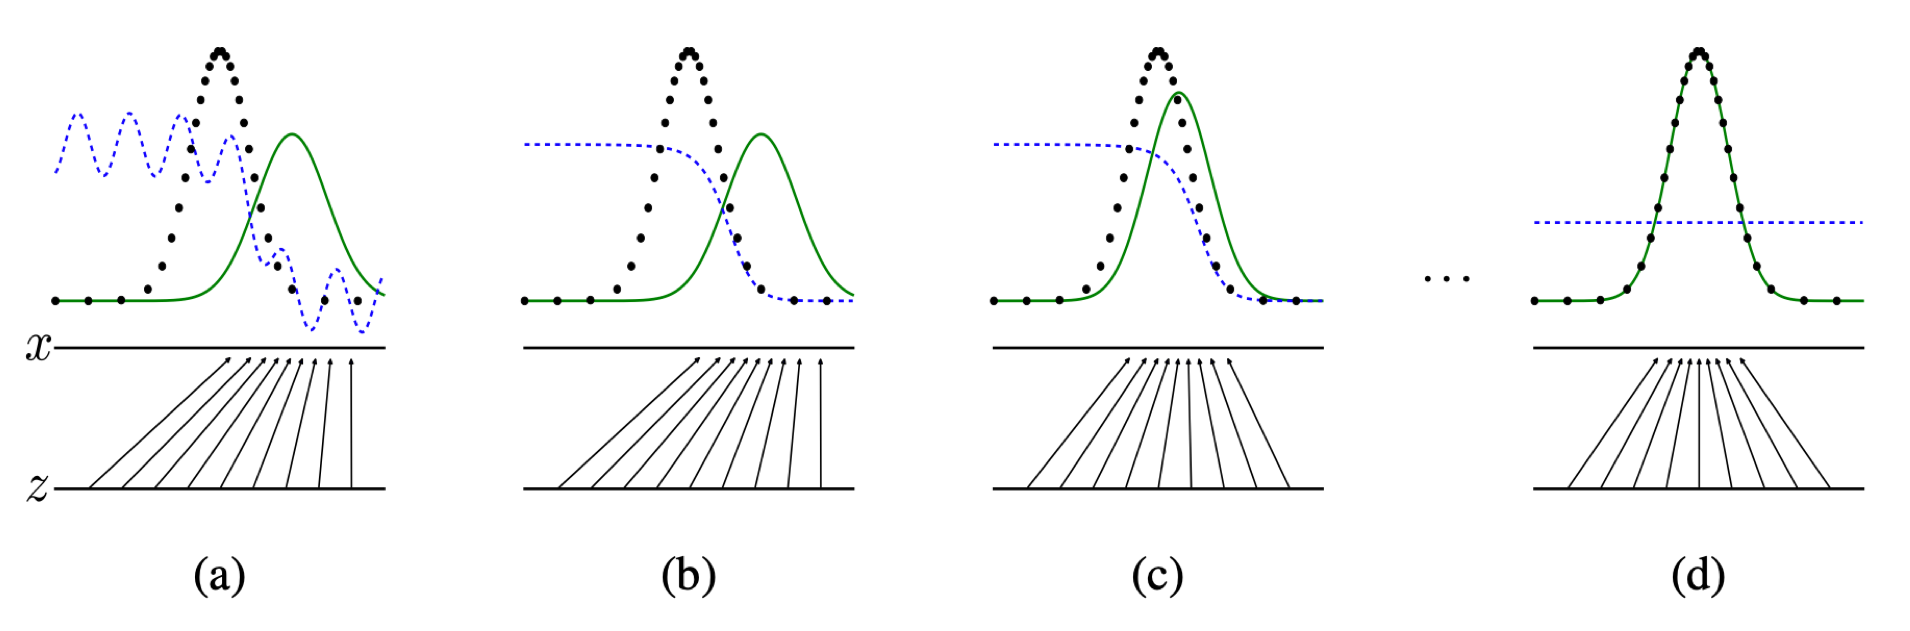
\includegraphics[scale=0.5]{images/test.png} %scale为图像尺寸,会latex的能看懂的吧
	\bicaption{测试图}{test figure} %这是双标图示
%\vspace{-0.5cm}  %调整图片与下文的垂直距离,视情况而定,这部分我给注释掉,需要的自己加入
\end{figure}

这是你的第一张图片~\cite{avriel2003nonlinear}

%这是没有超行和换等号的公式
\begin{equation} \label{equ:1.1}
\mathcal{L}_D= = \mathbb{E}_{x \sim p_data(x)} [\log{(D(x))}]+ \mathbb{E}_{z \sim p_z (z)} [\log⁡{(1-D(G(z))})]  
\end{equation}

这是你的第一个公式

%这是带换等号的公式
\begin{equation}\label{equ:1.2}
\begin{aligned}
\begin{split}
C(G) &= \max_D V(D,G) \\
&= \max_D \int_x p_{data}(x) \log{(D(x))} + p_g(x) \log{(1-D(x))} dx \\
&= \int_x p_{data}(x) \log{D_G^*(x)} + p_g(x) \log{(1-D_G^*(x))} dx \\
&= \int_x p_{data}(x) \log{(\frac{p_{data}(x)}{p_{data}(x)+p_g(x)})} + p_g(x) \log{(1-\frac{p_{data}(x)}{p_{data}(x)+p_g(x)})} dx \\
&= \int_x p_{data}(x) \log{(\frac{p_{data}(x)}{p_{data}(x)+p_g(x)})} + p_g(x) \log{(\frac{p_{g}(x)}{p_{data}(x)+p_g(x)})} dx \\
&= \int_x p_{data}(x) \log{(\frac{p_{data}(x)}{\frac{p_{data}(x)+p_g(x)}{2}})} + p_g(x) \log{(\frac{p_{g}(x)}{\frac{p_{data}(x)+p_g(x)}{2}})} dx - \log{4} \\
&= KL[p_{data}(x) \Vert \frac{p_{data}(x)+p_g(x)}{2}] + KL[p_g(x) \Vert \frac{p_{data}(x)+p_g(x)}{2}] - \log{4}
\end{split}
\end{aligned}
\end{equation}

这是你的第一个长公式

\begin{table}[!htb]
\centering
%\vspace{-0.2cm}  %调整图片与上文的垂直距离,视情况而定,这部分我给注释掉,需要的自己加入
\bicaption{生成对抗网络生成$28 \times 28 \times 1$的黑白图像的网络详细设计}{Detailed Network Design for Generating Adversarial Networks to Generate $28 \times 28 \times 1$ Black and White Images}
%\vspace{-0.15cm}  %调整标注与表格的垂直距离,视情况而定,这部分我给注释掉,需要的自己加入
\footnotesize
\begin{tabular}{cccc}
\hline
\multicolumn{2}{c}{\textbf{Generator}} & \multicolumn{2}{c}{\textbf{Discriminator}} \\ \hline
Layer & Shape & Layer & Shape \\
input layer & (B, 100) & input layer & (B, 28, 28, 1) \\
MLP-(100, 3136), BN, ReLU & (B, 3136) & CONV-(N64, K3, S2, P1), BN, LReLU & (B, 14, 14, 64)\\
Reshape & (B, 7, 7, 64) & CONV-(N64, K3, S2, P1), BN, LReLU & (B, 7, 7, 64)\\
DeCONV-(N64, K3, S2, P1), BN, ReLU & (B, 14, 14, 64) & CONV-(N128, K3, S2, P1), BN, LReLU & (B, 4, 4, 128)\\
CONV-(N128, K3, S1, P1), BN, ReLU & (B, 14, 14, 128) & CONV-(N128, K3, S1, P1), BN, LReLU & (B, 4, 4, 128)\\
DeCONV-(N64, K3, S2, P1), BN, ReLU & (B, 28, 28, 128) & Flatten & (B, 2048)\\
CONV-(N64, K3, S1, P1), BN, ReLU & (B, 28, 28, 64) & MLP-(2048, 1), BN, Sigmoid & (B, 1)\\
CONV-(N64, K3, S1, P1), BN, ReLU & (B, 28, 28, 64) \\
CONV-(N1, K3, S1, P1), BN, ReLU & (B, 28, 28, 1) \\ \hline
\end{tabular}
%\vspace{-0.5cm}  %调整表注与下文的垂直距离,视情况而定,这部分我给注释掉,需要的自己加入
\end{table}

这是你的第一张表格

\begin{minted}[
	frame=lines,
	framesep=2mm,
	baselinestretch=1.2,
	fontsize=\footnotesize,
	linenos
]{python}

def adaptive_instance_layer_norm(x, gamma, beta, smoothing=True, scope='instance_layer_norm'):
    with tf.variable_scope(scope):
        ch = x.shape[-1]
        eps = 1e-5
        # 计算Instance mean,sigma and ins
        ins_mean, ins_sigma = tf.nn.moments(x, axes=[1, 2], keep_dims=True)
        x_ins = (x - ins_mean) / (tf.sqrt(ins_sigma + eps))
        
        # 计算Layer mean,sigma and ln
        ln_mean, ln_sigma = tf.nn.moments(x, axes=[1, 2, 3], keep_dims=True)
        x_ln = (x - ln_mean) / (tf.sqrt(ln_sigma + eps))
        
        # 给定rho的范围,smoothing控制rho的弹性范围
        if smoothing:
            rho = tf.get_variable("rho", [ch], initializer=tf.constant_initializer(0.9),
                                  constraint=lambda x: tf.clip_by_value(x, 
                                  clip_value_min=0.0, clip_value_max=0.9))
        else:
            rho = tf.get_variable("rho", [ch], initializer=tf.constant_initializer(1.0),
                                  constraint=lambda x: tf.clip_by_value(x,
                                  clip_value_min=0.0, clip_value_max=1.0))

        # rho = tf.clip_by_value(rho - tf.constant(0.1), 0.0, 1.0)

        x_hat = rho * x_ins + (1 - rho) * x_ln

        x_hat = x_hat * gamma + beta

        return x_hat
\end{minted}

% 参考文献
{
\clearpage % 分页
\pagestyle{plain} % 这部分不需要页眉
\phantomsection % 使得hyperref目录能够跳转到正确的位置
\addcontentsline{toc}{section}{参考文献} % 添加到目录中
\setlength{\baselineskip}{18pt}
\nocite{*} % 添加所有文献
%\bibliographystyle{gbt7714-2005} % 样式
\bibliographystyle{bib/gbt7714-2005} % 样式
\bibliography{bib/ref.bib}    % 文献数据库,到bib/ref.bib文件中添加,用过Latex都会用的吧
}

% 攻读硕士学位期间的学术活动及成果情况
\pagestyle{plain}
\begin{achievement}
1)参加的学术交流与科研项目

\songti \fighao{
\begin{itemize}
	\item [(1)] 
		你做的第一个项目
	\item [(2)] 
		第二个项目
\end{itemize}
}

\heiti \xiaosihao{2)发表的学术论文(含专利和软件著作权)}
\setlength{\baselineskip}{20pt}

\fighao{
\begin{itemize}
	\item [(1)] 
Paper1
	\item [(2)] 
Paper2
\end{itemize}
}

\end{achievement}

\end{document}
